\chapter{Background and Related Work}

\section{Overview}

In this chapter, the concepts and definitions which are needed to implement the proposed system are identified. In the first section, the tools and concepts used from relational database management system and in the second section, the concepts in Blockchain technology are introduced. third section is also dedicated to discuss about the related work and the researches which have been done in this field and compare it with our proposed system.

\section{Temporal Databases}
Temporal database is any type of database that requires some aspect of time \cite {elmasri2010fundamentalsofdatabase} which in the proposed system, it is a way to store and manage historical records of the transactions.

%----------------------------------definition Temporal Database-----------------------------------------

\textbf {Definition 1. (Temporal Database)}:
Let $ r_i = \{r_1, r_2, ... , r_n \}$, be $n$ number of tables in the relational database $D$. Denote the attributes of each table as $attr(r_i)$. A temporal table denoted $r_i^T$ is a table with attributes $atr(r_i^T) = \{ (updated, deleted) \in \mathcal{T} \}\cup attr(r_i)$ where $\mathcal{T} = \{t_0,t_1,...,t_n\}$ is the time domain in which transactions on $r_i$ happened. A temporal database denoted $D^T$ is the result of augmenting $D$ by $r_i^T$:

\begin{center}
	{$D^T = D \cup \{{r_i^T}: r_i \in D \}$}
\end{center}

The temporal database $D^T$ contains the entire history of the records ever existed in $D$.

\textbf{Example 1.} Given the normal relational table $r_1$ (Table 2.1) and temporal table $r_1^T$ (Table 2.2), the $attr(r_1) = (id, item, value)$ and $attr(r_1^T)= (id, item, value, updated, deleted)$. The result of query $q_1 = \sigma_{id = 22}(r_1)$ is $\{(22,Pencil,7.50\$)\}$ and the result of same query on the temporal table $q_2 = \sigma_{id = 22}(r_1^T)$ is $\{(22,pencil,8.0\$,2018-03-21,NULL),(22,pencil,7.50\$,2018-03-30,NULL)\}$. Also the query $q_3 = \sigma_{id = 21}(r_1)$ results in $NULL$ however, the same query on the temporal table $q_4 = \sigma_{id = 21}(r_1^T)$ has the history of record with id = 21: $\{(21,ruler,3.25,2018-02-10,NULL),(21,ruler,3.25,NULL,2018-02-20)\}$.
\begin{center}

\begin{table}[t]
	\centering
	\caption{Normal Relational Table $r_1$}
	\begin{tabular}{p{4cm}p{4cm}p{4cm}}
		\hline
		id & item      & value  \\ \hline
		22 & Pencil    & 7.50\$ \\
		23 & Notebook & 12.0\$   \\ \hline
	\end{tabular}
\end{table}

\begin{table}[t]
	\centering
	\caption{Temporal Table $r_1^T$}
	\begin{tabular}{p{1cm}p{2cm}p{3cm}p{3cm}p{2cm}}
		\hline
		id & item      & value  & updated  & deleted\\ \hline
		21 & Ruler    & 3.25\$  & 2018-02-10  &  - \\  
		21 & Ruler    & 3.25\$  & -  &  2018-02-20 \\
		22 & Pencil    & 8.0\$  & 2018-03-21  &  - \\
		22 & Pencil    & 7.50\$  & 2018-03-30  &  -\\
		23 & Notebook & 12.0\$  & 2018-04-01 & - \\ \hline
	\end{tabular}
\end{table} 
\end{center}

%---------------------------------- End of Definition Temporal Database -----------------
%---------------------------------- Defintion Time Domain -------------------------------
\textbf{Definition2. (Time domain)}: 
The time domain $\mathcal{T}$ consists of discrete timestamps $t_0,t_1,...,t_n$ in which transactions on tables $r_i \in D$ happened. the range of time domain is: $\mathcal{T} = [t_0, \infty)$ where $t_0$ is the timestamp in which the first record added to the table $r_i$.
The time domain of a temporal table $r_i^T \in D^T $ is calculated by:

\begin{center}
	$\mathcal{T} = r_i^T[updated] \cup r_i^T[deleted]$
\end{center}
For example in the temporal table $r_1^T$ (Table 2.2), the time domain is:
$\mathcal{T} = [2018-02-10,2018-04-01]$.
%---------------------------------- End of Definition Time Domain -----------------------
%---------------------------------- Defintion Timestamps --------------------------------

\textbf{Definition 3. (Timestamps)}: A timestamp $t_i \in \mathcal{T}$ is a particular position in the time domain, in which particular transaction(s) happened. For example in the temporal table $r_1^T$ (Table 2.2), ``2018-03-30'' is a timestamp in which the record with ``id = 22'' updated.
%---------------------------------- End of Definition Timestamps ------------------------
%---------------------------------- Defintion Timeline ----------------------------------

\textbf{Definition 4. (Timeline)}: Let $u_i(t_j)$ be the total transactions on the tables $r_i \in D$ at timestamps $t_j \in \mathcal{T}$, where $i,j=\{0,1,...,n\}$. The $u_i(t_j)$ could be represented as an ordered set points on a vector. This vector is called a timeline for the transactions happened on $r_i \in D$. Figure x illustrates the concept of timeline.
\begin{figure}
	\label{fig:timeline}
	\centering
	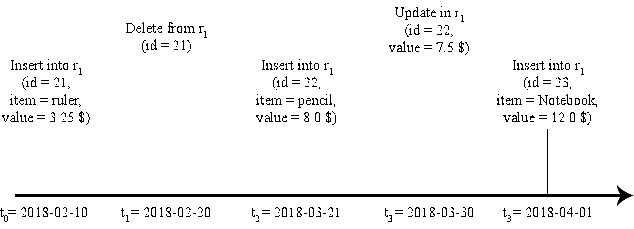
\includegraphics[width=\textwidth]{figs/timeline.pdf}
	\caption{Timeline.}
\end{figure}

%---------------------------------- End of Definition Timeline --------------------------
%---------------------------------- Defintion snapshot ----------------------------------
\textbf{Defionition 5. (Snapshot and snapshot-queries)}: Given a temporal table $r^T \in D^T$ and a timestamp $t \in \mathcal{T}$, we denote $s(t)$ to be the table instance that obtained by calculating the $\{max(r^T[m])|t : m\in r)\}-r^T[deleted]$ for $\mathcal{T}\leq t$. Note that $s(t) \in D^T$ but not necessarily $s(t) \in D$. A snapshot is a materialized version of $D(t) = \{s_1(t),s_2(t),...,s_n(t)\}$. A snapshot-query is an arbitrary relational query on $D(t)$.\\

We can construct the snapshots using simple windowing functions (as in supported
by PostgreSQL \cite{momjian2001postgresql}).

    \vspace{1em}
\begin{center}

{\small
	\begin{tabular}{|l|} \hline
		$\mathrm{snapshot}(r, t)$ = \\
		\verb|| \textsc{With} $T$ \textsc{as} ( \\
		\verb| | \textsc{select} id, $\{\mathrm{last\_value}(x) \mathrm{\ as\ } x:
		x\in attr(r)\}$ \textsc{over} $W$ \\
		\verb| | \textsc{from} $r^T$ \\
		\verb| | \textsc{where} updates $\leq t$ \\
		\verb| | \textsc{window} $W$ \textsc{as} 
		\textsc{partition by} id \textsc{order by} updates\\
		\verb|| ) \\
		\verb|| \textsc{select} id, $\{x: x\in attr(r)\}$ \textsc{from} $T$ \\
		\verb|| \textsc{where not} $T.$deleted \\ \hline
	\end{tabular}
}
\end{center}

The query $\mathrm{snapshot}(r, t)$ computes the snapshot of $r$ at timestamp
$t$ by applying the latest update of each tuple up to timestamp $t$, while
removing tuples that have been deleted.

%---------------------------------- End of Definition snapshot --------------------------


\section{Blockchain}
\textbf{Definition.(Cryptography)}:
Cryptography is a way of secure communication between parties in a network while adversaries might also be present. Using Cryptography, messages sent or received are encrypted so that the adversaries cannot read the normal form of the message. This communication is established through various steps such as cryptographic key assignment, encryption and decryption of messages or digitally signing a message and verifying the digital signatures.


\textbf{Definition.(Cryptographic Keys)}: Let $u$ be the authenticated user who is using database $D$. By the creation of the profile of $u$ in the system, a set of strings $<K_{priv},K_{pub}> \in \mathbf{N}^+$ is generated and assigned to the user where $K_{pub}$ is the public key that is accessible to everyone on the system, and $K_{priv}$ is the private key that is known only to $u$. These keys are used to encrypt/decrypt messages which is transmitted between the users.


\textbf{Definition.(Assymetric Encryption)}: Let $E$ be the encryption algorithm, $D$ be the decryption algorithm, m be the message which needs to be encrypted and c be the encrypted message. Given the cryptographic keys $<K_{pub}, K_{priv}>$, An encryption technique is said to be asymmetric if:

\begin{center}
	$c = E(K_{pub},m)$ and  $m = D(K_{priv},c)$
\end{center}
or
\begin{center}
	$c = E(K_{priv},m)$ and  $m = D(K_{pub},c)$
\end{center}
Therefore:
\begin{center}
	$D(E(m,K_{pub}),K_{priv}) = m$ 
\end{center}
and
\begin{center}
	$D(E(m,K_{priv}),K_{pub}) = m$
\end{center}
Note that, if $K_{pub}$ is known, and $E(K_{pub},m)$ is also known, in asymmetric encryption method, it is impossible to get $m$ without $K_{priv}$.

Figure x shows the basic steps to send and receive messages between two parties in a secure way by utilizing asymmetric encryption technique. [Figure and description to be added]

\textbf{Definition. (Hash function)}: Assume $m \in \mathcal{A}$ to be the message with an arbitrary size chosen from domain $\mathcal{A}$. $hash(m)\rightarrow sketch$ 
is a function that maps the $m$ of any size from domain $\mathcal{A}$ to a fixed size string (normally 256 bits) in a smaller domain $\mathcal{B}$.


\textbf{Definition. (Digital Signature)}: Digital signature is used to ensure that the digitally transfered data has not altered while transferring. Also it verifies whether or not the transfered data was submitted by a recognized source. \\
Let $m$ be the document which needs to be digitally signed and transfered. Denote $h$ as hash function, $E$ as encryption algorithm and $D$ as decryption algorithm. In order to digitally signing a document and verify a signature, following steps should be taken:
\begin{itemize}
	\item \textbf{Step 1.} $S_r = h(m)$
	\item \textbf{Step 2.} $c = E(S,K_{priv})$
	\item \textbf{Step 3.} $m$ and $c$ are sent
\end{itemize}
In order to verify:
\begin{itemize}
	\item \textbf{Step 1.} $m$ and $c$ are received
	\item \textbf{Step 2.} $S_t = h(m)$ is calculated
	\item \textbf{Step 3.} $S_r = D(c,K_{priv})$ is obtained
	\item \textbf{Step 4.} $m$ is valid if $S_t = S_r$ and invalid if $S_t \neq S_r$
\end{itemize}
Figure x depicts the steps that needs to be taken for digitally sign a document and verifying a digital signature.
\begin{figure}
	\label{fig:DigitalSignature}
	\centering
	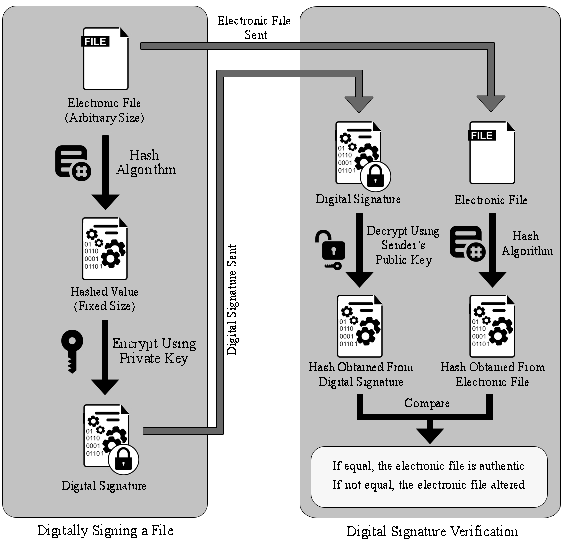
\includegraphics[width=\textwidth]{figs/digital_signature.pdf}
	\caption{Digital Signature Creation and Verification.}
\end{figure}
%---------------------------------- Defintion  ----------------------------------